\usetikzlibrary{arrows.meta,calc,patterns,shapes}
\providecommand{\computer}{%
    
\includegraphics[width=1cm,alt={computer}]{../common/Noun_project_216.pdf}
}
\providecommand{\switch}{%
    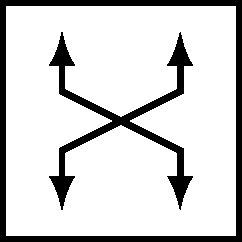
\includegraphics[width=0.9cm,alt={switch}]{../common/fig-switch.pdf}
}
\providecommand{\bigswitch}{%
    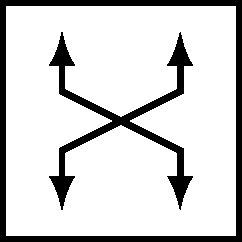
\includegraphics[width=1.4cm,alt={switch}]{../common/fig-switch.pdf}
}
\providecommand{\router}{%
    
\includegraphics[width=0.9cm,alt={router}]{../common/fig-router.pdf}
}



\begin{frame}\frametitle{flows / packets}
\begin{tikzpicture}
\tikzset{
    connect one/.style={draw,very thick,-Latex},
    computer/.style={inner sep=0mm,outer sep=0mm,execute at begin node={\computer}},
    switch/.style={inner sep=0mm,outer sep=0mm,execute at begin node={\switch}},
    big switch/.style={inner sep=0mm,outer sep=0mm,execute at begin node={\bigswitch}},
    packet/.style={minimum width=.4cm,minimum height=0.2cm,inner sep=0mm,outer sep=0mm,draw},
    packet lg/.style={minimum width=.6cm,minimum height=0.2cm,inner sep=0mm,outer sep=0mm,draw},
    c1c2/.style={fill=violet!40,draw=black,thin,slidealt=<2>{thick,draw=red}},
}
\node[computer] (c1) at (-5, 1) {};
\node at (c1) {1};
\node[big switch] (s1) at (-2,-.5) {};
\node[big switch] (s2) at (2,.5) {};
\node[computer] (c2) at (6, 2) {};
\node at (c2) {2};
\draw[connect one] (c1) -- (s1)
    node[above=0.05cm,sloped,packet,c1c2,pos=0.1] {}
    node[above=0.05cm,sloped,packet lg,c1c2,pos=0.5] {}
    node[above=0.05cm,sloped,packet,c1c2,pos=0.8] {};
\draw[connect one] (s1) -- (s2)
    node[above=0.05cm,sloped,packet,c1c2,pos=0.3] {}
    node[above=0.05cm,sloped,packet,c1c2,pos=0.8] {};
\draw[connect one] (s2) -- (c2)
    node[above=0.05cm,sloped,packet,c1c2,pos=0.2] {}
    node[above=0.05cm,sloped,packet lg,c1c2,pos=0.6] {};
\node[packet,c1c2,anchor=north east] at ([yshift=-.1cm,xshift=-.1cm]s1.north east) {};
\node[packet lg,c1c2,anchor=north east] at ([yshift=-.3cm,xshift=-.1cm]s1.north east) {};
%
\node[packet,c1c2,anchor=north east] at ([yshift=-.1cm,xshift=-.1cm]s2.north east) {};
\node[packet,c1c2,anchor=north east] at ([yshift=-.3cm,xshift=-.1cm]s2.north east) {};
\node[packet,c1c2,anchor=north east] at ([yshift=-.5cm,xshift=-.1cm]s2.north east) {};
\coordinate (box loc) at (-4, -1.5);
\tikzset{
    explain box/.style={
        overlay,draw=red, align=left, very thick, anchor=north west,at=(box loc)
    },
}
\begin{visibleenv}<1>
\node[explain box] {
    \textit{\myemph{flow}} of data between two machines \\
    ~ \\
    \textit{flow} is very general term \\
    will depend on context how it relates to \\
    connections, sockets, etc.
};
\end{visibleenv}
\begin{visibleenv}<2>
\node[explain box] {
    \textit{\myemph{flow}} of data between two machines \\
    ~ \\
    possibly divided up into pieces, \\
    called \textit{\myemph{packets}}, \textit{\myemph{frames}}, \textit{\myemph{segments}} \\
    (which name is best depends on context)
};
\end{visibleenv}
\end{tikzpicture}
\end{frame}

\begin{frame}\frametitle{(de)multiplexing}
\begin{tikzpicture}
\tikzset{%
    connect one/.style={draw,very thick,-Latex},
    connect one lg/.style={draw,line width=1mm,-Latex},
    connect one sm/.style={draw,thick,-Latex},
    computer/.style={inner sep=0mm,outer sep=0mm,execute at begin node={\computer}},
    switch/.style={inner sep=0mm,outer sep=0mm,execute at begin node={\switch}},
    big switch/.style={inner sep=0mm,outer sep=0mm,execute at begin node={\bigswitch}},
    packet/.style={minimum width=.4cm,minimum height=0.2cm,inner sep=0mm,outer sep=0mm,draw},
    packet lg/.style={minimum width=.6cm,minimum height=0.2cm,inner sep=0mm,outer sep=0mm,draw},
    c1c2/.style={fill=violet!40,draw=black,thin},
    c3c4/.style={pattern=checkerboard,pattern color=green!70,draw=black,thin},
    buffer 1/.style={slidealt=<5>{draw=red,thick},slidealt=<8>{draw=red,thick}},
    buffer 2/.style={slidealt=<5>{draw=red,thick}},
}
\node[computer] (c1) at (-5, 1) {};
\node at (c1) {1};
\node[big switch,slidealt=<3-4>{fill=red!10},slidealt=<6>{fill=red!10}] (s1) at (-2,-.5) {};
\node[big switch,slidealt=<3-4>{fill=red!10}] (s2) at (2,.5) {};
\node[computer] (c2) at (6, 2) {};
\node at (c2) {2};
\node[computer] (c3) at (-5, -1) {};
\node at (c3) {3};
\node[computer] (c4) at (6, 0) {};
\node at (c4) {4};
\draw[connect one] (c3) -- (s1)
    node[above=0.05cm,sloped,packet lg,c3c4,pos=0.2] {}
    node[above=0.05cm,sloped,packet,c3c4,pos=0.7] {};
\draw[connect one] (c1) -- (s1)
    node[above=0.05cm,sloped,packet,c1c2,pos=0.1] {}
    node[above=0.05cm,sloped,packet lg,c1c2,pos=0.5] {}
    node[above=0.05cm,sloped,packet,c1c2,pos=0.8] {};
\draw[connect one,slidealt={<2>{draw=red,ultra thick}}] (s1) -- (s2)
    node[above=0.05cm,sloped,packet,c1c2,pos=0.3] {}
    node[above=0.05cm,sloped,packet,c3c4,pos=0.6] {}
    node[above=0.05cm,sloped,packet,c1c2,pos=0.8] {};
\draw[connect one sm] (s2.north east) -- (c2)
    node[above=0.05cm,sloped,packet,c1c2,pos=0.2] {}
    node[above=0.05cm,sloped,packet lg,c1c2,pos=0.6] {};
\draw[connect one sm] (s2.south east) -- (c4)
    node[above=0.05cm,sloped,packet,c3c4,pos=0.2] {}
    node[above=0.05cm,sloped,packet lg,c3c4,pos=0.6] {};
\node[packet,c3c4,buffer 1,anchor=north east] at ([yshift=-.1cm,xshift=-.1cm]s1.north east) {};
\node[packet,c1c2,buffer 1,anchor=north east] at ([yshift=-.3cm,xshift=-.1cm]s1.north east) {};
\node[packet lg,c1c2,buffer 1,anchor=north east] at ([yshift=-.5cm,xshift=-.1cm]s1.north east) {};
\begin{visibleenv}<8>
\node[packet,c3c4,buffer 1,anchor=north east,opacity=0.9,draw=red] at ([yshift=-.7cm,xshift=-.1cm]s1.north east) {};
\node[packet lg,c1c2,buffer 1,anchor=north east,opacity=0.8,draw=red] at ([yshift=-.9cm,xshift=-.1cm]s1.north east) {};
\node[packet,c1c2,buffer 1,anchor=north east,opacity=0.7,draw=red] at ([yshift=-1.1cm,xshift=-.1cm]s1.north east) {};
\node[packet,c1c2,buffer 1,anchor=north east,opacity=0.5,draw=red] at ([yshift=-1.3cm,xshift=-.1cm]s1.north east) {};
\node[packet,c1c2,buffer 1,anchor=north east,opacity=0.3,draw=red] at ([yshift=-1.3cm,xshift=-.1cm]s1.north east) {};
\node[packet,c1c2,buffer 1,anchor=north east,opacity=0.1,draw=red] at ([yshift=-1.5cm,xshift=-.1cm]s1.north east) {};
\end{visibleenv}
\node[packet,c1c2,buffer 2,anchor=north east] at ([yshift=-.1cm,xshift=-.1cm]s2.north east) {};
\node[packet,c1c2,buffer 2,anchor=north east] at ([yshift=-.3cm,xshift=-.1cm]s2.north east) {};
\node[packet,c1c2,buffer 2,anchor=north east] at ([yshift=-.5cm,xshift=-.1cm]s2.north east) {};
\node[packet lg,c3c4,buffer 2,anchor=south east] at ([yshift=.1cm,xshift=-.1cm]s2.south east) {};
\coordinate (box loc) at (-4, -1.5);
\tikzset{%
    explain box/.style={%
        overlay,draw=red, align=left, very thick, anchor=north west,at=(box loc)
    },
}
\begin{visibleenv}<2>
\node[explain box] {%
    two or more flows can \\
    share one or more links
};
\end{visibleenv}
\begin{visibleenv}<3>
\node[explain box] {%
    left switch \textit{\myemph{multiplexes}} the two flows onto one link \\
    right switch \textit{\myemph{demultiplexes}} them to separate them
};
\end{visibleenv}
\begin{visibleenv}<4>
\node[explain box] {%
    this picture: multiplexed by dividing up \textit{time} on link
};
\end{visibleenv}
\begin{visibleenv}<5>
\node[explain box] {%
    switches usually have \textit{\myemph{buffers}} (also called \textit{\myemph{queues}}) \\
    hold waiting packets \\
    ~ \\
    absorbs temporary ``bursts'' where packets come faster \\
    than outgoing link can handle
        % FIXME: diagram of packets coming in over time
};
\end{visibleenv}
\begin{visibleenv}<6-7>
\node[explain box] {%
    incomplete list of causes of `bursts': \\
    ~ \\
    \myemph<6>{multiple unsynchronized flows} \\
    \myemph<7>{fast links produce packets faster for slow can send}
};
\end{visibleenv}
\begin{visibleenv}<8>
\node[explain box] {%
    if buffer full, switch must \textit{\myemph{drop}} packets \\
    will happen eventually if overall rate faster than outgoing link \\
    ~\\
    scenario is called \textit{\myemph{congestion}}
};
\end{visibleenv}
\end{tikzpicture}
\end{frame}

\begin{frame}\frametitle{buffer usage: fast to slow, store + forward}
\begin{tikzpicture}
\tikzset{
    axis/.style={draw,thick,-Latex},
    scale mark/.style={draw,thin},
    scale label/.style={font=\small},
    packet/.style={ultra thick,fill=violet!20},
    y=.6cm
}
\begin{scope} % input
    \begin{scope}[shift={(0.1, 0)}]
        \clip (0, 0) rectangle (12.5, 3.2);
        \draw[packet] (0, 0) coordinate (A recv start) rectangle (2, 3) node[midway] {packet A};
        \draw[packet] (2, 0) rectangle (4, 3) node[midway] {packet B};
        \draw[packet] (4, 0) rectangle (6, 3) node[midway] {packet C};
        \draw[packet] (10, 0) rectangle (12, 3) node[midway] {packet D};
    \end{scope}
    \draw[axis] (0, 0) -- ++ (12.5, 0);
    \draw[axis] (0, 0) -- ++ (0, 3.3)
        node[midway,left=.5cm,align=right] { input };
    \draw[scale mark] (0, 3) -- ++ (.25, 0) node[pos=0,left,scale label] {capacity};
\end{scope} 
\begin{scope}[shift={(0, -5)}]% buffer usage
    \begin{scope}
        \clip (0,0) rectangle (12.5, 4);
        \draw[violet, ultra thick] (0, 0) -- (0.1, 0) -- (0.1, 1) -- (2.1, 1) -- (2.1, 2) -- (4.1, 2) -- (4.1, 3)
            -- (5.1, 3) -- (5.1, 2) -- (8.1, 2) -- (8.1, 1) -- (10.1, 1) -- (10.1, 2) -- 
            (11.1, 2) -- (11.1, 1) -- (14, 1);
    \end{scope}
    \draw[axis] (0, 0) -- ++ (12.5, 0);
    \draw[axis] (0, 0) -- ++ (0, 4.3)
    node[midway,left=.5cm,align=right] (usage label) { buffer \\ reserved };
    \node[font=\small,anchor=north,align=center] at (usage label.south) {
        packets
    };
    \draw[scale mark] (0, 1) -- ++ (.25, 0) node[pos=0,left,scale label] {1};
    \draw[scale mark] (0, 2) -- ++ (.25, 0) node[pos=0,left,scale label] {2};
    \draw[scale mark] (0, 3) -- ++ (.25, 0) node[pos=0,left,scale label] {3};
    \draw[scale mark] (0, 4) -- ++ (.25, 0) node[pos=0,left,scale label] {4};

\end{scope}
\begin{scope}[shift={(0, -8)}] % output
    \begin{scope}
        \clip (0, 0) rectangle (12.5, 2.2);
        \begin{scope}[shift={(2.1, 0)}]
            \draw[packet] (0, 0) coordinate (A send start) rectangle (3, 2) node[midway] {packet A};
            \draw[packet] (3, 0) rectangle (6, 2) node[midway] {packet B};
            \draw[packet] (6, 0) rectangle (9, 2) node[midway] {packet C};
            \draw[packet] (10, 0) rectangle (13, 2) node[midway] {packet D};
        \end{scope}
    \end{scope}
    \draw[axis] (0, 0) -- ++ (12.5, 0);
    \draw[axis] (0, 0) -- ++ (0, 2.3)
        node[midway,left=.5cm,align=right] { output };
    \draw[scale mark] (0, 2) -- ++ (.25, 0) node[pos=0,left,scale label] {capacity};
\end{scope}
\begin{visibleenv}<2>
    \draw[draw=red,dotted,ultra thick,Latex-Latex] (A send start) -- ++(-2cm, 0);
    \draw[draw=red,dotted,ultra thick] (A send start) -- ++(0cm, 6cm);
    \draw[draw=red,dotted,ultra thick] ([xshift=-2cm]A send start) -- ++(0cm, 6cm);
    \node[draw=red,ultra thick,align=left,fill=white,anchor=west] at  (2.2, -3) {
        \textit{store and forward} \\
        switch stores whole packet in buffer\\
        then sends it out \\
        ~ \\
        our default in this class
    };
\end{visibleenv}
\end{tikzpicture}
\end{frame}

\begin{frame}\frametitle{buffer usage: fast to slow, cut-through}
\begin{tikzpicture}
\tikzset{
    axis/.style={draw,thick,-Latex},
    scale mark/.style={draw,thin},
    scale label/.style={font=\small},
    packet/.style={ultra thick,fill=violet!20},
    y=.6cm
}
\begin{scope} % input
    \begin{scope}[shift={(0.1, 0)}]
        \clip (0, 0) rectangle (12.5, 3.2);
        \draw[packet] (0, 0) coordinate (A recv start) rectangle (2, 3) node[midway] {packet A};
        \draw[packet] (2, 0) rectangle (4, 3) node[midway] {packet B};
        \draw[packet] (4, 0) rectangle (6, 3) node[midway] {packet C};
        \draw[packet] (10, 0) rectangle (12, 3) node[midway] {packet D};
    \end{scope}
    \draw[axis] (0, 0) -- ++ (12.5, 0);
    \draw[axis] (0, 0) -- ++ (0, 3.3)
        node[midway,left=.5cm,align=right] { input };
    \draw[scale mark] (0, 3) -- ++ (.25, 0) node[pos=0,left,scale label] {capacity};
\end{scope} 
\begin{scope}[shift={(0, -5)}]% buffer usage
    \begin{scope}
        \clip (0,0) rectangle (12.5, 4);
        \draw[violet, ultra thick] (0, 0) -- (0.1, 0) -- (0.1, 1) -- (2.1, 1) -- (2.1, 2) -- 
            (3.6, 2) -- (3.6, 1) -- (4.1, 1) -- (4.1, 2) -- (6.6, 2) -- (6.6, 1) --
            (9.6, 1) -- (9.6, 0) -- (10.1, 0) -- (10.1, 1) -- (13.6, 1) -- (13.6, 0);
    \end{scope}
    \draw[axis] (0, 0) -- ++ (12.5, 0);
    \draw[axis] (0, 0) -- ++ (0, 4.3)
    node[midway,left=.5cm,align=right] (usage label) { buffer \\ reserved };
    \node[font=\small,anchor=north,align=center] at (usage label.south) {
        packets
    };
    \draw[scale mark] (0, 1) -- ++ (.25, 0) node[pos=0,left,scale label] {1};
    \draw[scale mark] (0, 2) -- ++ (.25, 0) node[pos=0,left,scale label] {2};
    \draw[scale mark] (0, 3) -- ++ (.25, 0) node[pos=0,left,scale label] {3};
    \draw[scale mark] (0, 4) -- ++ (.25, 0) node[pos=0,left,scale label] {4};

\end{scope}
\begin{scope}[shift={(0, -8)}] % output
    \begin{scope}
        \clip (0, 0) rectangle (12.5, 2.2);
        \begin{scope}[shift={(0.6, 0)}]
            \draw[packet] (0, 0) coordinate (A send start) rectangle (3, 2) node[midway] {packet A};
            \draw[packet] (3, 0) rectangle (6, 2) node[midway] {packet B};
            \draw[packet] (6, 0) rectangle (9, 2) node[midway] {packet C};
            \draw[packet] (10, 0) rectangle (13, 2) node[midway] {packet D};
        \end{scope}
    \end{scope}
    \draw[axis] (0, 0) -- ++ (12.5, 0);
    \draw[axis] (0, 0) -- ++ (0, 2.3)
        node[midway,left=.5cm,align=right] { output };
    \draw[scale mark] (0, 2) -- ++ (.25, 0) node[pos=0,left,scale label] {capacity};
\end{scope}
\begin{visibleenv}<1>
    \draw[draw=red,dotted,ultra thick] (A send start) -- ++(-.5cm, 0);
    \draw[draw=red,dotted,ultra thick] (A send start) -- ++(0cm, 6cm);
    \draw[draw=red,dotted,ultra thick] ([xshift=-.5cm]A send start) -- ++(0cm, 6cm);
    \node[draw=red,ultra thick,align=left,fill=white,anchor=west] at  (2.2, -3) {
        \textit{cut-through} forwarding \\
        switch sends packet out as it's being received \\
        ~ \\
        uncommon and much more complex to implement
    };
\end{visibleenv}
\end{tikzpicture}
\end{frame}
% FIXME: multiplexing at end hosts
